\documentclass[11pt,a4paper]{article}
\usepackage[T1]{fontenc}
\usepackage[utf8]{inputenc}
\usepackage[polish]{babel}
\usepackage{mathptmx}
\usepackage[margin=2.5cm]{geometry}
\usepackage{amsmath,graphicx,booktabs,float,caption,microtype}
\usepackage[hidelinks]{hyperref}
\setlength{\parindent}{0pt}
\setlength{\parskip}{4pt}
\setlength{\tabcolsep}{6pt}
\renewcommand{\arraystretch}{1.12}
\captionsetup{font=small,labelfont=bf}
\hypersetup{
  pdftitle={SIGK -- Projekt 2: Rozjaśnianie zdjęć},
  pdfauthor={Aleksandra Buczma, Aleksandra Samsel},
  pdfsubject={Zespół Olé}
}

\begin{document}
\begin{center}
  {\LARGE\bfseries SIGK -- Projekt 2}\par
  \vspace{4pt}
  {\large Rozjaśnianie zdjęć przy słabym oświetleniu}\par
  \vspace{4pt}
  \textbf{Zespół Olé}\quad Aleksandra Buczma, Aleksandra Samsel
\end{center}

\begingroup\small
\setlength{\intextsep}{3pt}
\captionsetup{skip=3pt}
\section*{Architektura sieci neuronowej}
NAF-U-Net rozjaśnia zdjęcia i usuwa szum. Wejście jest najpierw wzmacniane
o 3 EV w przestrzeni liniowej. Sieć przewiduje poprawkę RGB, którą dodaje
do wstępnie rozjaśnionego obrazu. Model ma cztery poziomy kodera i dekodera
oraz \(11{,}57\) mln parametrów. Dekoder zwiększa rozdzielczość przez
\texttt{PixelShuffle} i dodaje cechy z odpowiedniego poziomu kodera.

\section*{Dane}
Z RAISE wybrano pierwszych 100 zdjęć wnętrz z aparatu Nikon D7000.
W kolejności pliku CSV przeznaczono 70 zdjęć do treningu, 10 do walidacji
i ostatnie 20 do testu.

Z plików NEF wywołano obrazy referencyjne sRGB oraz obrazy liniowe do symulacji.
Ekspozycję zmniejszono o 3 EV, dzieląc sygnał przez 8. Dodano szum Poissona
(\(\alpha=0{,}001\)) i Gaussa (\(\sigma=0{,}005\)), po czym zastosowano
korekcję gamma (\(\gamma=2{,}2\)) i zapisano wejście jako 8-bitowy RGB.

\section*{Funkcja straty i uczenie}
Strata Charbonniera mierzy błąd pikseli RGB i ogranicza wpływ dużych odchyleń.
SSIM wspiera zachowanie struktury, a cechy VGG-16 tekstury. Składnik lumy
dopasowuje lokalną jasność do wzorca.
\[
\mathcal{L}=\mathcal{L}_{\mathrm{Charb}}+
0{,}10(1-\mathrm{SSIM})+0{,}20\mathcal{L}_{\mathrm{luma}}+
0{,}02\mathcal{L}_{\mathrm{VGG}}.
\]
Trenowano przez 50 epok optymalizatorem AdamW na fragmentach
\(256\times256\) w partiach po 8. Współczynnik uczenia zmniejszano
kosinusowo od \(10^{-3}\) do \(10^{-6}\).

\begin{figure}[H]
\centering
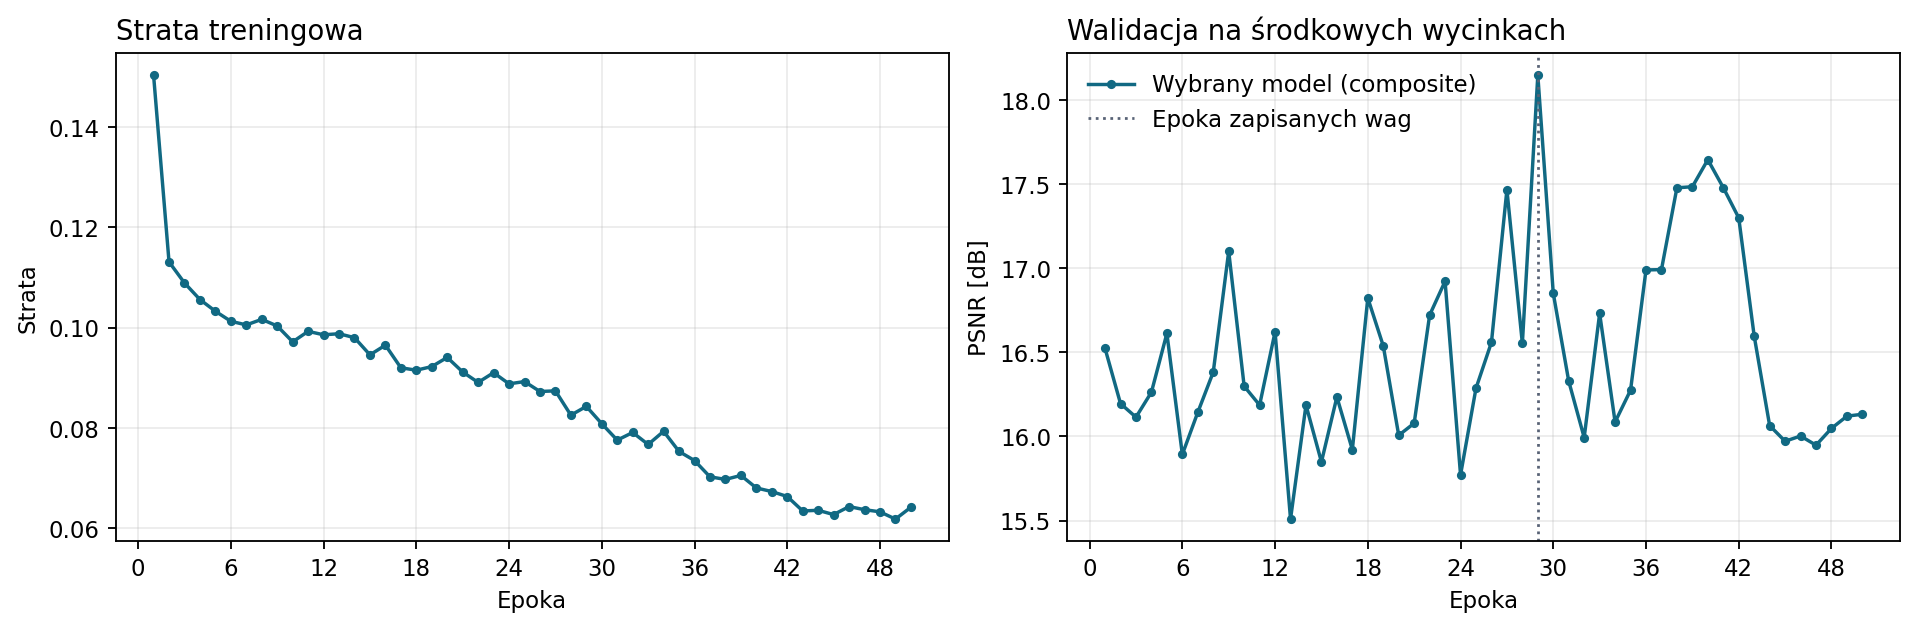
\includegraphics[width=0.89\linewidth]{images/training_curves.png}
\caption{Strata treningowa oraz PSNR na środkowych wycinkach walidacyjnych
\(512\times512\). Najlepsza epoka 29 (18,15 dB).}
\end{figure}
\endgroup

\clearpage
\begingroup
\setlength{\intextsep}{5pt}
\captionsetup{skip=5pt}
\section*{Wyniki}
Jako metodę odniesienia zastosowano wyrównanie histogramu składowej Y
w przestrzeni YCbCr. Sieć przetwarzała zdjęcia w kafelkach \(512\times512\)
z marginesem kontekstu do 32 pikseli. PSNR, SSIM i LPIPS (AlexNet) obliczono
dla pełnych obrazów względem wzorca i uśredniono osobno dla zbioru testowego
i walidacyjnego.

\begin{table}[H]
\centering\small
\begin{tabular}{@{}lrrrrr@{}}
\toprule
Metoda & Pocz. współcz. uczenia & Epoka & PSNR [dB] \(\uparrow\) & SSIM \(\uparrow\) & LPIPS \(\downarrow\) \\
\midrule
\multicolumn{6}{@{}l}{\textit{Test na 20 zdjęciach}} \\
Wyrównanie histogramu & - & - & 11,28 & 0,1528 & 1,0739 \\
NAF-U-Net, strata złożona & \(10^{-3}\) & 29 & \textbf{21,88} & \textbf{0,7015} & \textbf{0,3035} \\
\midrule
\multicolumn{6}{@{}l}{\textit{Walidacja na 10 zdjęciach}} \\
Strata złożona & \(10^{-3}\) & 29 & 15,25 & \textbf{0,4487} & \textbf{0,5125} \\
Strata złożona & \(10^{-3}\) & 50 & 14,26 & 0,4344 & 0,5172 \\
Strata Charbonniera z SSIM & \(10^{-3}\) & 40 & 14,39 & 0,4392 & 0,5451 \\
Strata złożona & \(3\cdot10^{-4}\) & 17 & \textbf{15,64} & 0,4373 & 0,5389 \\
\bottomrule
\end{tabular}
\caption{Średnie wyniki na pełnych zdjęciach RAISE.}
\end{table}

\textbf{Dodatkowe eksperymenty.}
Porównano wagi z epok 29 i 50. W dwóch osobnych treningach przy tym samym
podziale danych pominięto składniki lumy i VGG-16 lub zmniejszono początkowy
współczynnik uczenia dla straty złożonej. Niższy współczynnik dał najwyższy
walidacyjny PSNR. W teście użyto wag z epoki 29, które dały najwyższy SSIM
i najniższy LPIPS w walidacji.

W teście sieć poprawiła wszystkie trzy metryki dla każdego zdjęcia względem
wyrównania histogramu. Średni zysk PSNR wyniósł 10,61 dB (od 2,37 do 25,98 dB).

\subsection*{Porównanie obrazów}
\begin{figure}[H]
\centering
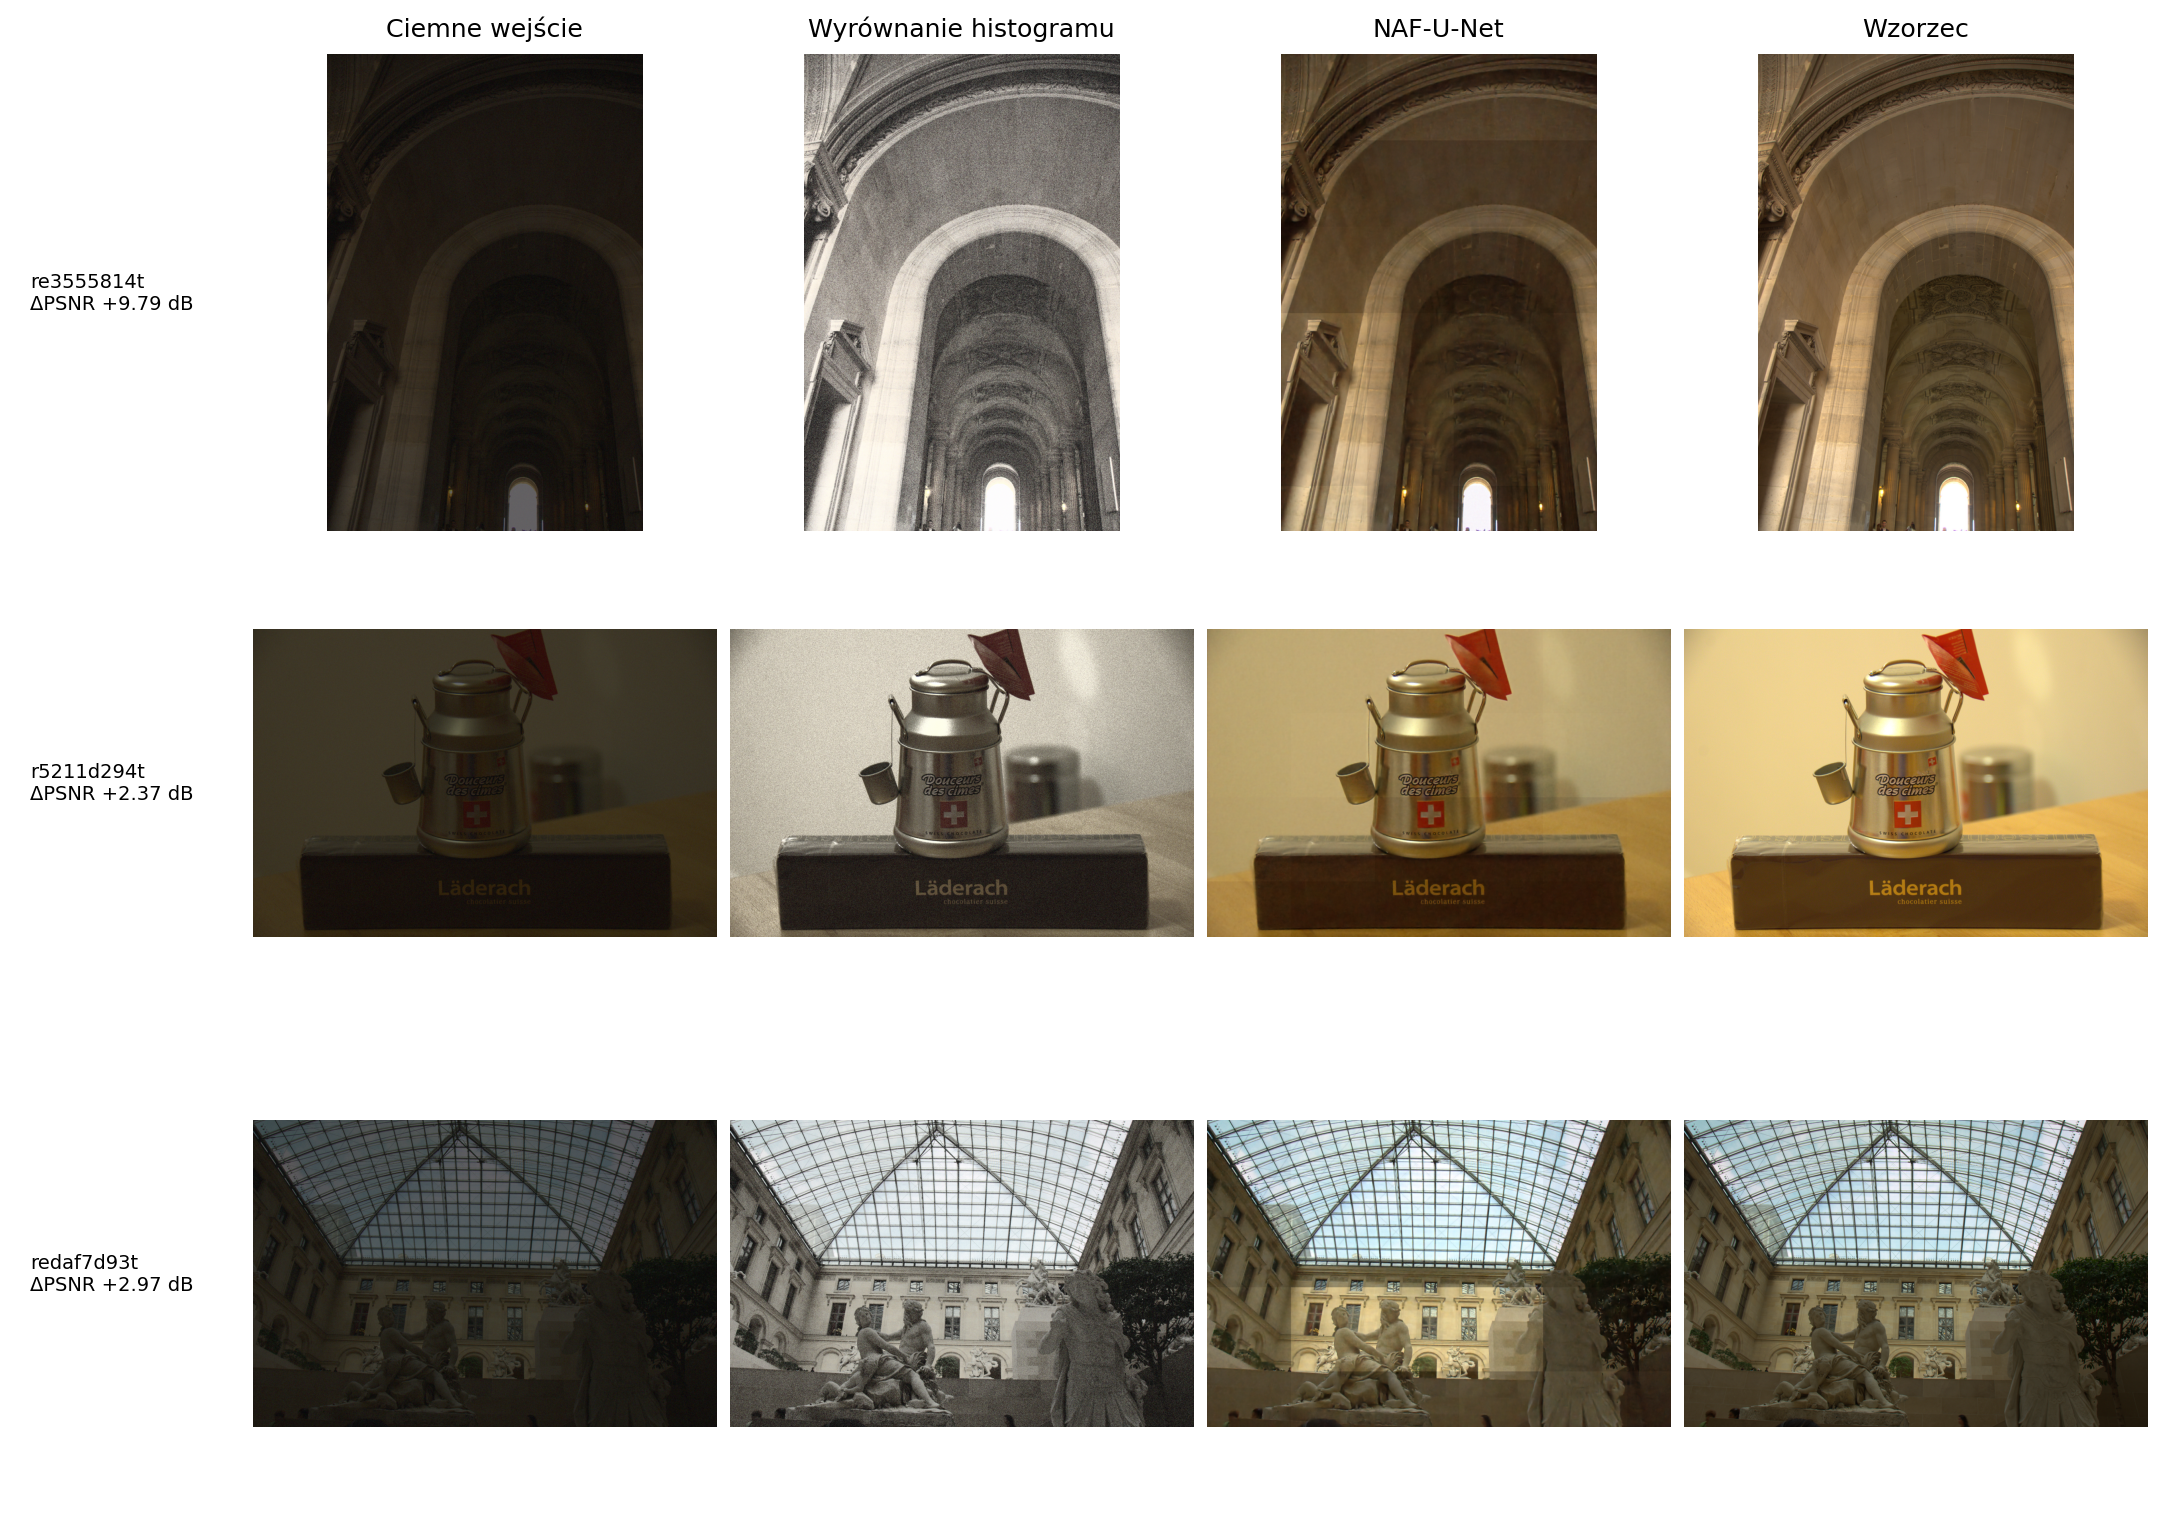
\includegraphics[width=0.77\linewidth]{images/photo_examples.png}
\caption{Pełne kadry trzech zdjęć testowych. \(\Delta\mathrm{PSNR}\) to
różnica między wynikiem NAF-U-Net a wyrównaniem histogramu.}
\end{figure}

Wyrównanie histogramu uwidacznia szum, szczególnie na kamiennym sklepieniu.
Sieć lepiej odtwarza ciepły odcień kamienia, czerwień etykiety
i niebieskawy kolor szyb.
\endgroup

\clearpage
\subsection*{Zbliżenia}
\begin{figure}[H]
\centering
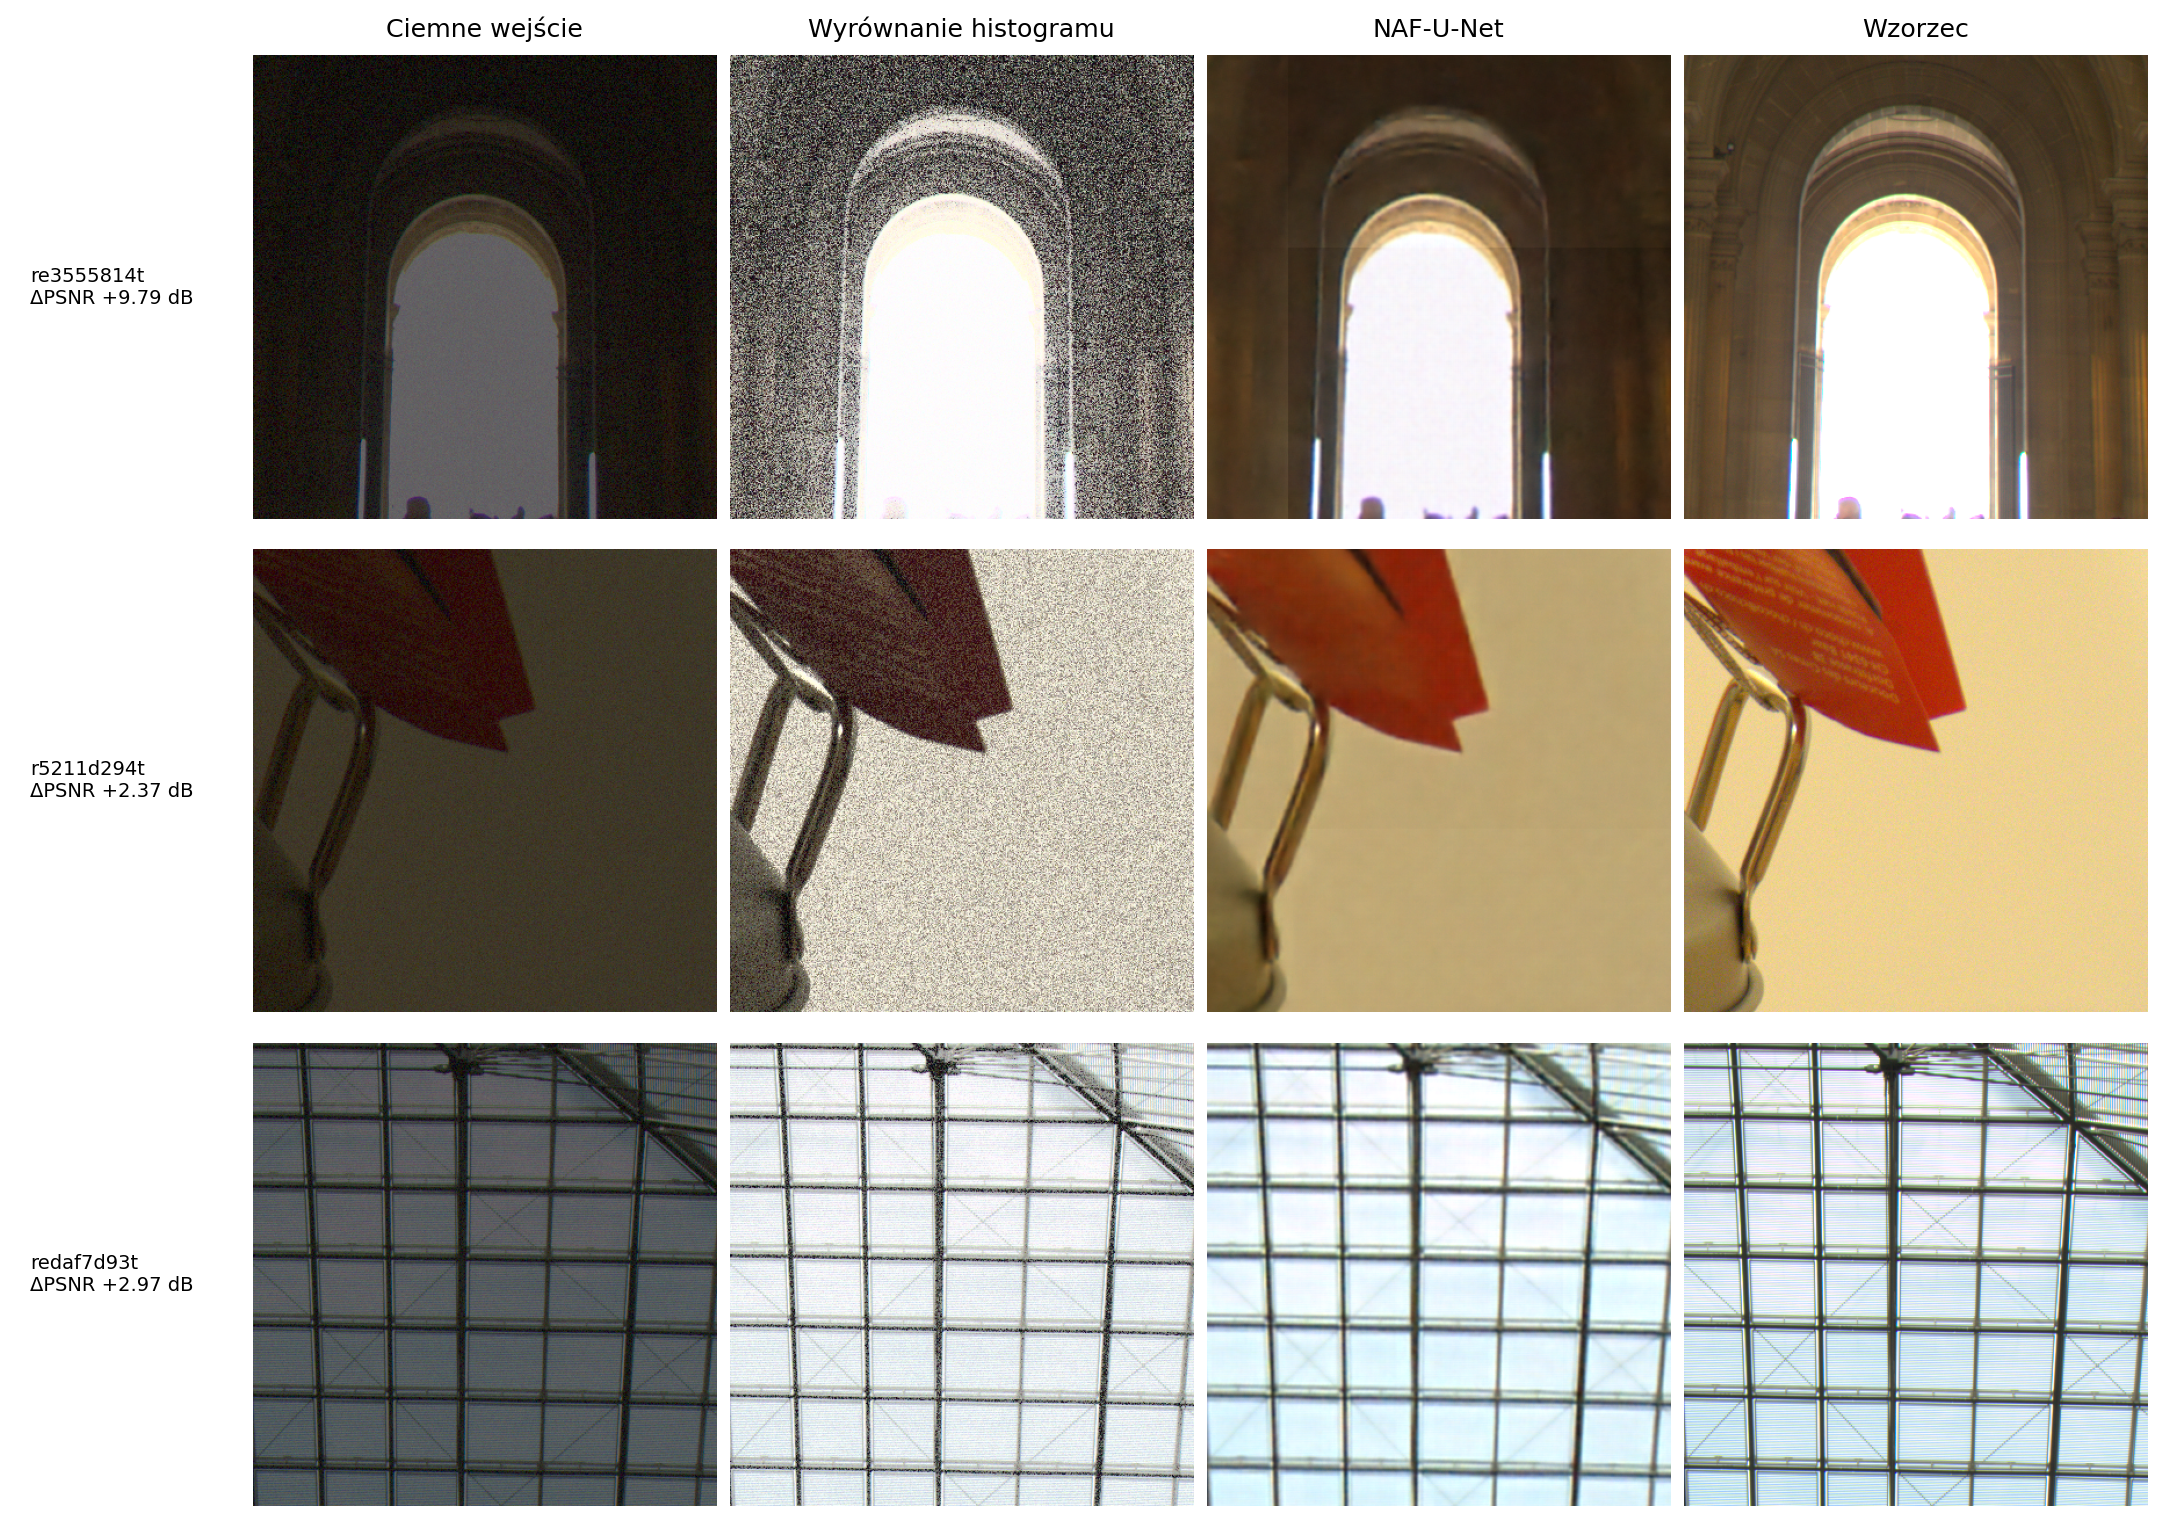
\includegraphics[width=\linewidth]{images/photo_details.png}
\caption{Te same obszary \(400\times400\) pikseli dla wejścia, obu metod
i wzorca. Kolejność zdjęć jak w porównaniu pełnych kadrów.}
\end{figure}

Na zbliżeniach sieć wygładza drobny nadruk na czerwonej etykiecie
i cienkie ukośne linie w szybach. Przy sklepieniu w rekonstrukcji widać
skok jasności w miejscu granicy kafelków. Jasne przejście w głębi sceny
pozostaje bliskie bieli również we wzorcu.

W całym zbiorze testowym co najmniej jeden kanał RGB osiągał wartość
\(\geq 0{,}99\) średnio dla 2,58\% pikseli we wzorcu, 4,49\% po wyrównaniu
histogramu i 0,86\% po rekonstrukcji siecią. Sieć odtwarzała więc mniej
pikseli bliskich nasycenia niż występowało w zdjęciach wzorcowych.

\subsection*{Wnioski}
Dla badanych zdjęć przyciemnionych o 3 EV model lepiej rozjaśnia obraz,
oddaje kolory i ogranicza szum niż wyrównanie histogramu. Największe
widoczne ograniczenia to wygładzanie drobnych detali i miejscowe granice
kafelków.

{\footnotesize\textbf{Źródła}\quad
\href{https://iris.unitn.it/handle/11572/122245}{RAISE (Dang-Nguyen i in., 2015)},
\href{https://www.ecva.net/papers/eccv_2022/papers_ECCV/papers/136670017.pdf}{NAFNet (Chen i in., 2022)},
\href{https://ece.uwaterloo.ca/~z70wang/publications/ssim.pdf}{SSIM (Wang i in., 2004)},
\href{https://arxiv.org/abs/1801.03924}{LPIPS (Zhang i in., 2018)}.}
\end{document}
